\documentclass[a4paper]{article}

\usepackage[english]{babel}
\usepackage[utf8x]{inputenc}
\usepackage{amsmath}
\usepackage{amsfonts}
\usepackage{graphicx}
\usepackage[colorinlistoftodos]{todonotes}

\title{CS 5785 -- Applied Machine Learning -- Lec.\ 14}
\author{Prof.\ Nathan Kallus, Cornell Tech\\Scribe: TBD}
\date{Oct.\ 19, 2017}

\begin{document}
\maketitle
\section{Procrustes Distance}

\subsection{Motivation}

The \emph{Procrustes distance} is a measure of dissimilarity defined on a pair of landmark datasets with known correspondences.  For instance, you might have spatial coordinates such as handwriting or GPS traces that you'd like to compare after finding the best alignment between them.  
Fig.~\ref{fig:signatures} shows an example of some handwriting data that we may wish to compare.

The method is named after a figure from Greek mythology, described as follows:
\begin{quote}
In Greek mythology, Procrustes or ``the stretcher [who hammers out the metal],'' also known as Prokoptas or Damastes ``subduer,'' was a rogue smith and bandit from Attica who physically attacked people by stretching them or cutting off their legs, so as to force them to fit the size of an iron bed. In general, when something is Procrustean, different lengths or sizes or properties are fitted to an arbitrary standard. [Wikipedia]
\end{quote}

\begin{figure}
\centering
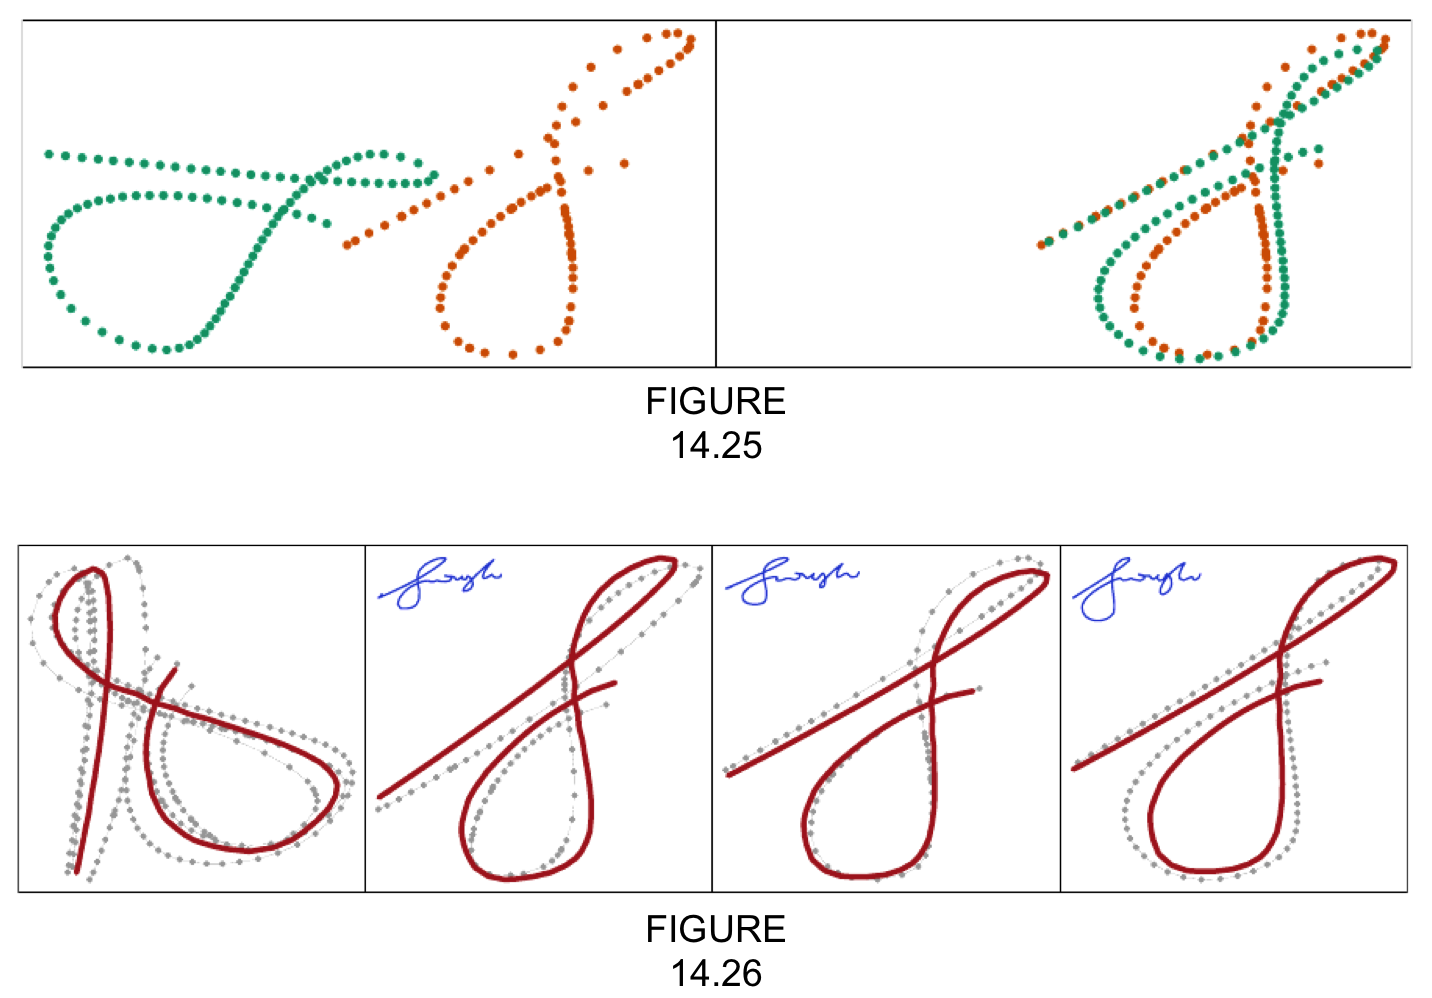
\includegraphics[width=1.0\textwidth]{fig14_26.png}
\caption{\label{fig:signatures}Procrustes alignment of handwritten symbols.  Top: Two sets of landmarks are captured on a digitizing tablet, with set 1 shown in green and set 2 shown in orange.  We assume they have known correspondences and we solve for the rigid transformation that best aligns the two point sets.}
\end{figure}


\subsection{Procrustes Alignment}
We have two sets of landmarks (or points) stored in the $N \times 2$ matrices $\mathbf{X}_1$ and $\mathbf{X}_2$, respectively.  The example from HTF has $N=96$.  We assume the points are \emph{in correspondence}, i.e., the landmark in the $i$th row of $\mathbf{X}_1$ corresponds to the landmark in the $i$th row of $\mathbf{X}_2$. In practice, if you were given two point sets like the ones in Fig.~\ref{fig:signatures}, you'd need to solve for the correspondences, which in general means finding the permutation between them while dealing with additions, deletions and noise.  In this lecture, we put this issue aside and focus instaed on finding the best alignment between the point sets.

The Procrustes alignment is the \emph{rigid transformation} that minimizes the following expression:
$$
\underset{\mu, R}{\min} {\|\mathbf{X}_2 - (\mathbf{X}_1\mathbf{R} + \vec{1}\mu^\top) \|}_F
$$
$\vec{1}$ is a vector of 1s and the subscript $F$ stands for the Frobenius norm which is given by
$$
\|\mathbf{A}\|^2_F = tr(\mathbf{A}^{\top} \mathbf{A})
$$
which is equivalent to the sum of the square of all the entries in $\mathbf{A}$.  $\mathbf{R}$ is a $2 \times 2$ rotation matrix and $\mu$ is a $2 \times 1$ translation vector. Since this is a rigid transformation, we don't allow scaling, stretching or shearing.  Only rotations and translations are allowed. Generalizations to more flexible transformations, including \emph{similarity} or \emph{affine} are straightforward, but we won't cover them here.

The $2\times 2$ rotation matrix $\mathbf{R}$ is specified by a single parameter $\theta$:
$$
\mathbf{R}(\theta) = \begin{bmatrix} {\cos\theta} & {-\sin\theta} \\ {\sin\theta} & {\cos\theta} \end{bmatrix}
$$
The matrix product $\mathbf{X}_1\mathbf{R}$ applies a rotation of $\theta$ to each row of $\mathbf{X}_1$.  The outer product
 $\vec{1}\mu^\top$, which has size $N\times 2$, copies the translation vector $N$ times.  Thus the quantity $\mathbf{X}_1\mathbf{R} + \vec{1}\mu^\top$ represents the rotated and translated version of $\mathbf{X}_1$ that we wish to be as close as possible to $\mathbf{X}_2$.

\subsection{Solution}

First compute the means of each point set and call them $\bar{x}_1$ and $\bar{x}_2$.  Let $\tilde{\mathbf{X}}_1, \tilde{\mathbf{X}}_2$ denote centered (i.e., mean-subtracted) versions of $\mathbf{X}_1$ and $\mathbf{X}_2$.  That leaves us to solve for $\mathbf{R}$, or equivalently, $\theta$.  Now compute the SVD of the inner product of the centered matrices:
$$
\tilde{\mathbf{X}}_1^\top \tilde{\mathbf{X}}_2 = \mathbf{UDV}^\top
$$
One can show the solution for $\mathbf{R}$ is given by:
$$
\hat{\mathbf{R}} = \mathbf{UV}^\top,\quad \hat{\mu} = \bar{x}_2 - \hat{\mathbf{R}}\bar{x}_1
$$
In this expression for $\mathbf{R}$, we effectively set $\mathbf{D}=\mathbf{I}$ in the SVD which yields the rotation $\mathbf{R}$ closest to the best affine (linear) alignment.  We skip the proof, which is based on differentiating the cost function w.r.t.\ $\theta$.

The singular values appearing on the diagonal of $\mathbf{D}$ represent stretching along the $x$ and $y$ axes.  We know that $\mathbf{U}$ and $\mathbf{V}$ are orthogonal, which means we can interpret them as rotation matrices.  When operating on a 2D vector, the product of the three matrices $\mathbf{UDV}^\top$ can be regarded as the following sequence of operations: rotate by some angle, scale by some amount horizontally and vertically, rotate by a second angle.  Forcing $\mathbf{D}$ to be the identity matrix eliminates the stretching part and just leaves the rotation part.

Procrustes alignment is often used as a component of shape-based recognition systems.


\section{Classical Multidimensional Scaling (MDS)}
Fig.~\ref{fig:dissimil} shows a table of dissimilarities between 11 countries obtained via a political science survey.  As an example, the low value of 2.17 for FRA-BEL indicates that the respondents regarded France and Belgium as highly similar.

\begin{figure}
\centering
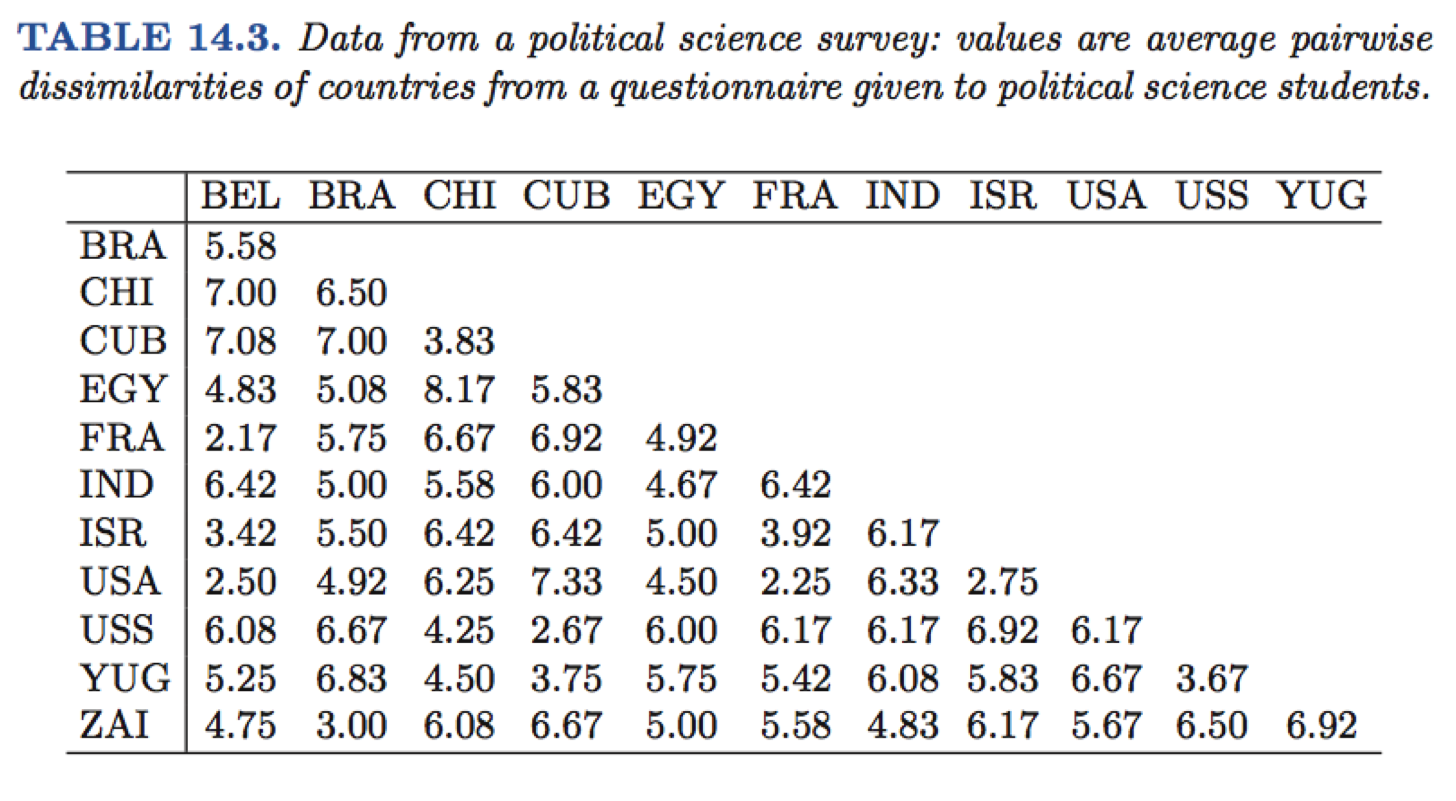
\includegraphics[width=1.0\textwidth]{table14_3.png}
\caption{\label{fig:dissimil}Table of dissimilarities}
\end{figure}

If we wanted to perform clustering on this dataset, we can't use $K$-means here because we don't have direct access to vector representations of the countries.  As discussed earlier, we could instead use $K$-medoids to cluster the data.  But what if we actually want to estimate a vectorial representation for the data?  That is the goal of MDS.

Given an input of $N \times N$ dissimilarity matrix $D$, MDS provides us a set of $N$ $k$-dimensional points that could have given rise to $D$.  In principle, one could approach this problem by a succession of triangulation steps to solve for the relative location of all the points.  The SVD provides us a more elegant solution.

As described in Ripley (1995), we start by converting the dissimilarity matrix into an inner product matrix.  For any symmetric matrix $\mathbf{T}$, we can define $\mathbf{T}'$ as follows:
$$
\mathbf{T}' = -\frac{1}{2} \left[\mathbf{T}-\frac{(\mathbf{T}\vec{1})\vec{1}^\top}{N}-\frac{\vec{1}(\mathbf{T}\vec{1})^\top}{N}+\frac{\vec{1}^\top\mathbf{T}\vec{1}}{N^2}\right]
$$
where $\vec{1}$ is a length $N$ column vector of $1s$.  Pre- or post-multiplication by a vector of 1s is a linear algebraic trick for summing the rows or columns of a matrix, respectively.  Sandwiching $\mathbf{T}$ in the form $\vec{1}^\top\mathbf{T}\vec{1}$ simply adds up all its entries.

The resulting matrix $\mathbf{T}'$ has the following properties:
\begin{enumerate}
\item If $\mathbf{T}$ was formed by computing pairwise Euclidean distances between the $x_i$ for $i=1,\ldots,N$, then $\mathbf{T}'$ contains the corresponding inner products, i.e. $\mathbf{T}' = \mathbf{XX}^\top$. \textcolor{red}{(\textbf{X} is centered)}
\item We can use the SVD to obtain the factorization $\mathbf{T}'=\mathbf{XX}^\top$. The rows of $\mathbf{X}$ will contain the coordinates we seek.
\end{enumerate}
\textcolor{red}{Explain how to use SVD to get X.}

The proof of this is based on the following observation.  Recalling that $\|a\|^2 = a^\top a$, the squared distance between two points $x_i$ and $x_j$ is expressed as

\textcolor{red}{Add that $x_i, x_j is centered$}

$$
\|x_i-x_j\|^2 = (x_i-x_j)^\top(x_i-x_j) = \|x_i\|^2 + \|x_j\|^2 - 2x_i^\top x_j
$$
The transformation of $\mathbf{T}$ into $\mathbf{T}'$ effectively subtracts off the two terms corresponding to the norms of $x_i$ and $x_j$ and just leaves us with the inner product term, $x_i^\top x_j$.

Because $\mathbf{T}'$ can be expressed as $\mathbf{XX}^\top$, it is positive semidefinite, which means all of its eigenvalues are nonnegative.  This also means we can interpret it as a covariance matrix.  As a result, MDS has strong conceptual links to PCA. 

Fig.~\ref{fig:mds1} shows the result of MDS applied to the country dissimilarity data using the first two recovered coordinates.  It's up to us to interpret of the axes in this plot, e.g., one axis might capture capitalist vs.\ communist and the other rich vs.\ poor.

\begin{figure}
\centering
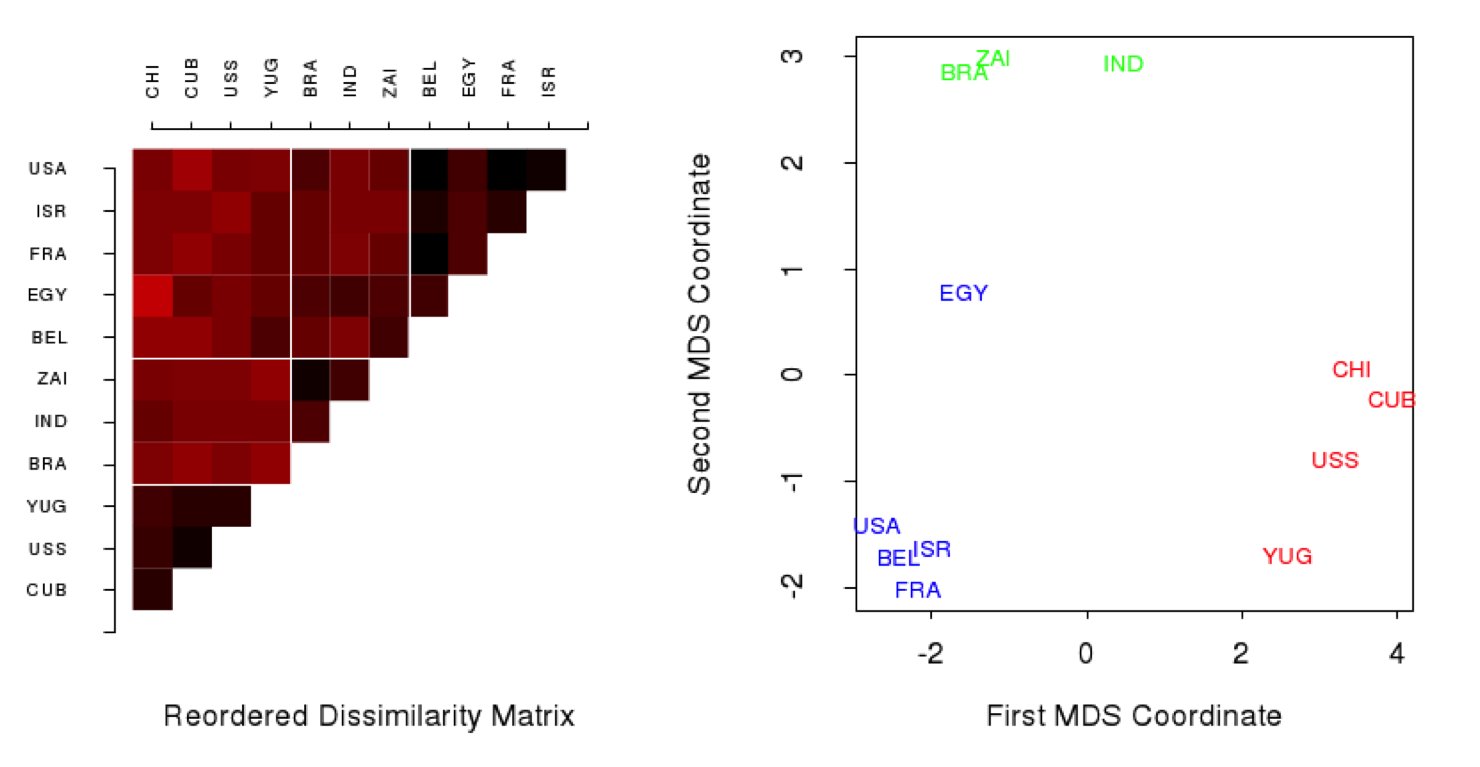
\includegraphics[width=1.0\textwidth]{mds.png}
\caption{\label{fig:mds1}Classical MDS applied to country dissimilarity data.}
\end{figure}

As a more concrete example, suppose you are given a distance matrix (in miles) between 9 cities, as shown in Fig.~\ref{fig:mds2}, and you want to construct a map (2D, in this case) of the city locations that are consisten with this distance matrix.  We approach this with the caveat that the reconstruction (or embedding or coordinatization) we find will, in general, be related to the original city locations by an unknown rotation, translation and reflection, since those operations don't affect the pairwise distances.

\begin{figure}
\centering
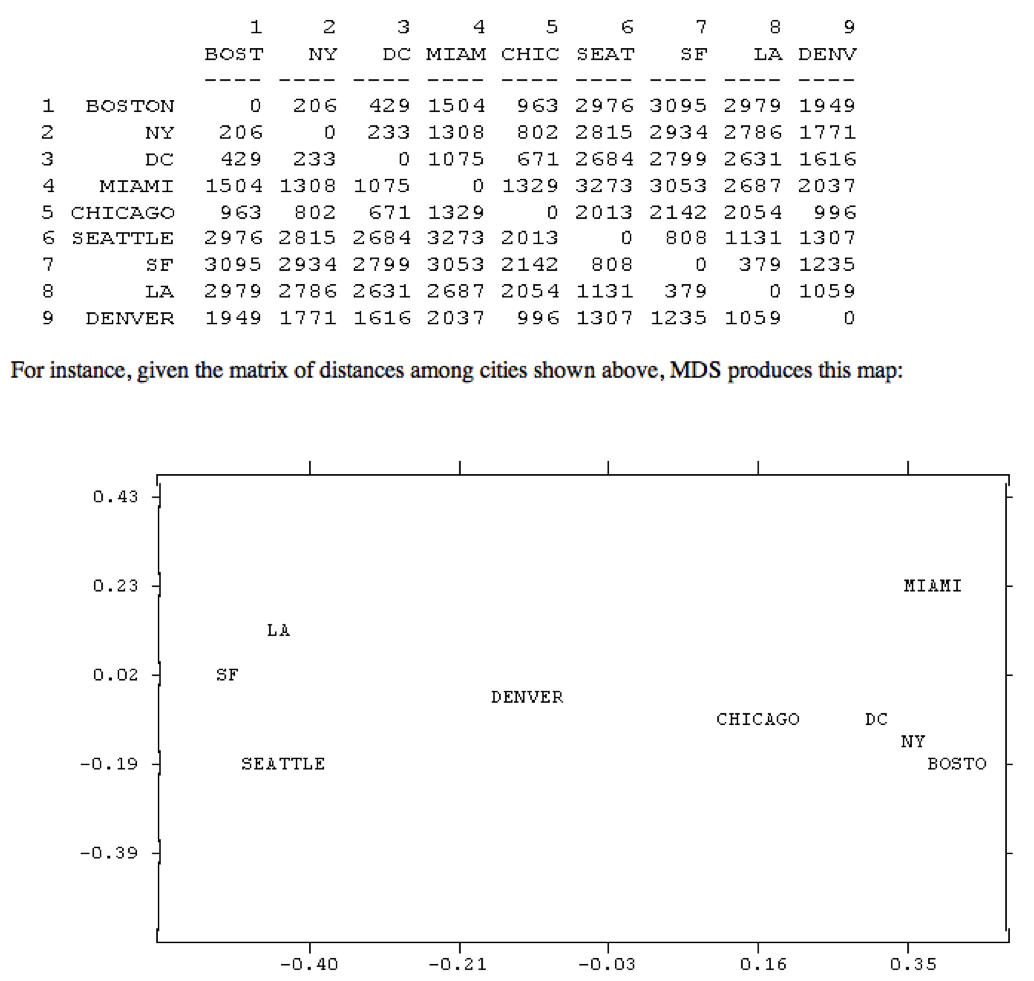
\includegraphics[width=1.0\textwidth]{mds2.png}
\caption{\label{fig:mds2}MDS applied to a mileage chart.  The resulting 2D embedding is quite reasonable, apart from a north-south reflection. [http://www.analytictech.com/borgatti/mds.htm]}
\end{figure}


\end{document}
